\documentclass[journal,12pt,twocolumn]{IEEEtran}

\usepackage{enumitem}
\usepackage{amsmath}
\usepackage{amssymb}
\usepackage{gensymb}
\usepackage{graphicx}
\usepackage{txfonts}         
\usepackage{listings}
\usepackage{lstautogobble}
\usepackage{mathtools}
\usepackage{bm}
\usepackage{hyperref}
\usepackage{polynom}
\usepackage{siunitx}
\usepackage{verbatim}

\newcommand{\solution}{\noindent \textbf{Solution: }}
\providecommand{\pr}[1]{\ensuremath{\Pr\left(#1\right)}}
\providecommand{\brak}[1]{\ensuremath{\left(#1\right)}}
\providecommand{\cbrak}[1]{\ensuremath{\left\{#1\right\}}}
\providecommand{\sbrak}[1]{\ensuremath{\left[#1\right]}}
\providecommand{\mean}[1]{E\left[ #1 \right]}
\providecommand{\var}[1]{\mathrm{Var}\left[ #1 \right]}
\providecommand{\der}[1]{\mathrm{d} #1}
\providecommand{\gauss}[2]{\mathcal{N}\ensuremath{\left(#1,#2\right)}}
\providecommand{\mbf}{\mathbf}
\providecommand{\abs}[1]{\left\vert#1\right\vert}
\providecommand{\norm}[1]{\left\lVert#1\right\rVert}
\providecommand{\z}[1]{{\mathcal{Z}}\{#1\}}
\providecommand{\ztrans}{\overset{\mathcal{Z}}{ \rightleftharpoons}}

\providecommand{\parder}[2]{\frac{\partial}{\partial #2} \brak{#1}}

\let\StandardTheFigure\thefigure
\let\vec\mathbf

%\numberwithin{equation}{section}
%\renewcommand{\thefigure}{\theenumi}
%\renewcommand\thesection{\arabic{section}}

\newcommand{\myvec}[1]{\ensuremath{\begin{pmatrix}#1\end{pmatrix}}}
\newcommand{\mydet}[1]{\ensuremath{\begin{vmatrix}#1\end{vmatrix}}}
\newcommand{\define}{\stackrel{\triangle}{=}}

\DeclareMathOperator*{\argmin}{arg\,min}
\DeclareMathOperator*{\argmax}{arg\,max}

\makeatletter
\def\pld@CF@loop#1+{%
    \ifx\relax#1\else
        \begingroup
          \pld@AccuSetX11%
          \def\pld@frac{{}{}}\let\pld@symbols\@empty\let\pld@vars\@empty
          \pld@false
          #1%
          \let\pld@temp\@empty
          \pld@AccuIfOne{}{\pld@AccuGet\pld@temp
                            \edef\pld@temp{\noexpand\pld@R\pld@temp}}%
           \pld@if \pld@Extend\pld@temp{\expandafter\pld@F\pld@frac}\fi
           \expandafter\pld@CF@loop@\pld@symbols\relax\@empty
           \expandafter\pld@CF@loop@\pld@vars\relax\@empty
           \ifx\@empty\pld@temp
               \def\pld@temp{\pld@R11}%
           \fi
          \global\let\@gtempa\pld@temp
        \endgroup
        \ifx\@empty\@gtempa\else
            \pld@ExtendPoly\pld@tempoly\@gtempa
        \fi
        \expandafter\pld@CF@loop
    \fi}
\def\pld@CMAddToTempoly{%
    \pld@AccuGet\pld@temp\edef\pld@temp{\noexpand\pld@R\pld@temp}%
    \pld@CondenseMonomials\pld@false\pld@symbols
    \ifx\pld@symbols\@empty \else
        \pld@ExtendPoly\pld@temp\pld@symbols
    \fi
    \ifx\pld@temp\@empty \else
        \pld@if
            \expandafter\pld@IfSum\expandafter{\pld@temp}%
                {\expandafter\def\expandafter\pld@temp\expandafter
                    {\expandafter\pld@F\expandafter{\pld@temp}{}}}%
                {}%
        \fi
        \pld@ExtendPoly\pld@tempoly\pld@temp
        \pld@Extend\pld@tempoly{\pld@monom}%
    \fi}
\makeatother

\lstset {
	frame=single, 
	breaklines=true,
	columns=fullflexible,
	autogobble=true
}             
                               
\title{Assignment 2 \\ \Large EE3900: Linear Systems and Signal Processing \\ \large Indian Institute of Technology Hyderabad}
\author{Ankit Saha \\ \normalsize AI21BTECH11004 \\ \vspace*{20pt} \normalsize 25 Sep 2022 \\ \vspace*{20pt} \Large Discrete-time Signal Processing \\ \large Oppenheim and Schafer}


\begin{document}

	\maketitle
	
	\textbf{Problem 2.3} By direct evaluation of the convolution sum, determine the step response of a linear time-invariant system whose impulse response is
	\begin{align}
		h(n) = a^{-n} u(-n) \qquad 0 < a < 1
	\end{align}
	
	\solution 
	We have
	\begin{align}
		x(n) = u(n) = 
		\begin{cases}
			1 & n \ge 0 \\
			0 & n < 0
		\end{cases}
	\end{align}
	
	and
	\begin{align}
		h(n) = a^{-n}u(-n) = 
		\begin{cases}
			0 & n > 0 \\
			a^{-n} & n \le 0
		\end{cases}
	\end{align}
	
	Their convolution is given by
	\begin{align}
		y(n) &= x(n) * h(n) \\
		&= \sum_{k=-\infty}^\infty h(k) x(n-k) \\
		&= \sum_{k=-\infty}^0 a^{-k} u(n-k) \\
		&= \sum_{k=0}^\infty a^k u(n+k)
	\end{align}
	
	If $n \ge 0$ then $n + k \ge 0 ~\forall k \ge 0$
	\begin{align}
		y(n) &= \sum_{k=0}^\infty a^k \\
		&= \frac{1}{1-a} &&\because 0<a<1
	\end{align}
	
	Else, if $n < 0$ then $n + k \ge 0 ~\forall k \ge -n > 0$
	\begin{align}
		y(n) &= \sum_{k=-n}^\infty a^k \\
		&= \frac{a^{-n}}{1-a} &&\because 0<a<1
	\end{align}
	
	Therefore, for $0 < a < 1$
	\begin{align}
		y(n) = 
		\begin{cases}
			\dfrac{1}{1-a} & n \ge 0 \\
			\dfrac{a^{-n}}{1-a} & n < 0
		\end{cases}
	\end{align}
	
	\begin{figure}[!ht]
		\centering
		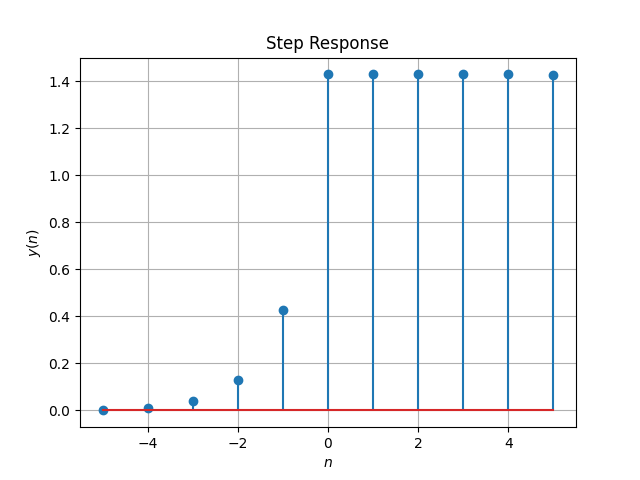
\includegraphics[width=\columnwidth]{./figs/fig-1.png}
		\caption{Plot of the step response for the given impulse response for $a = 0.3$}
		\label{fig-1}	
	\end{figure}

\end{document}